\subsection{Analyisis}


\begin{figure}[ht]
	\centering
	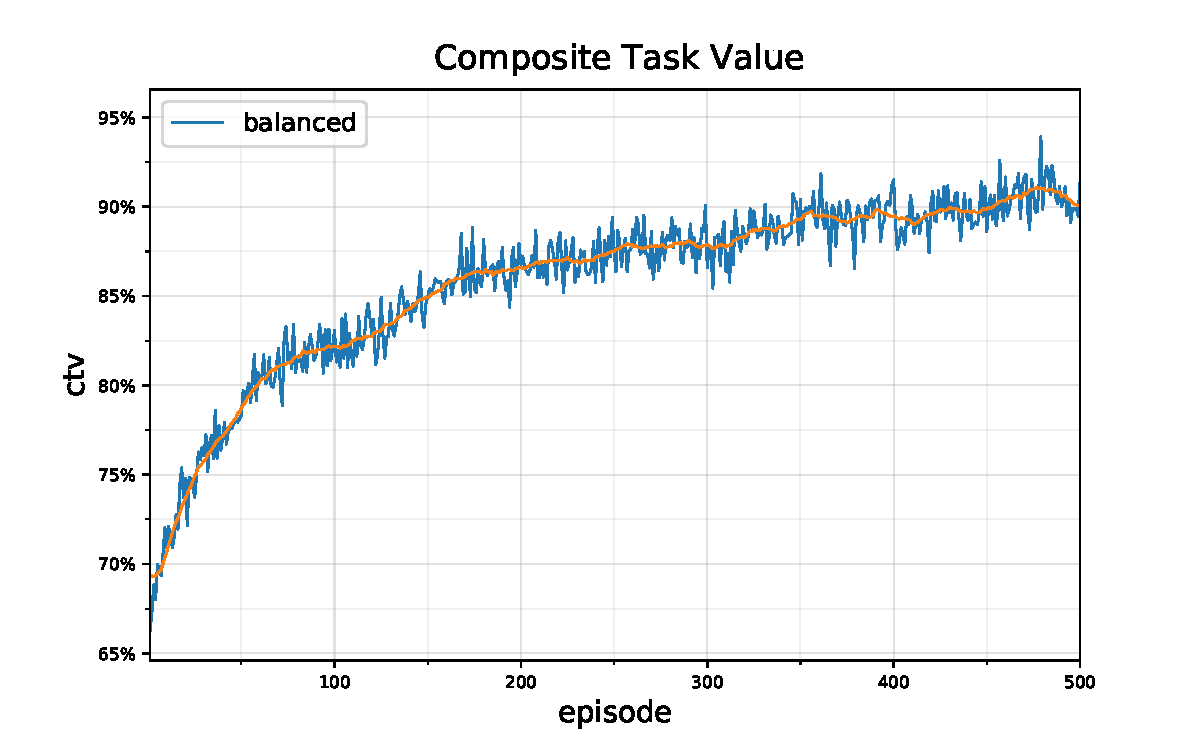
\includegraphics[width=0.7\linewidth]{5_ctv-optimal-ctv}
	\captionsetup{labelfont=bf,singlelinecheck=on}
	\caption{System utility comparison to the system optimal in the optimal system}
	\label{fig:5_ctv-optimal-ctv}
\end{figure}
\begin{figure}[ht]
	\centering
	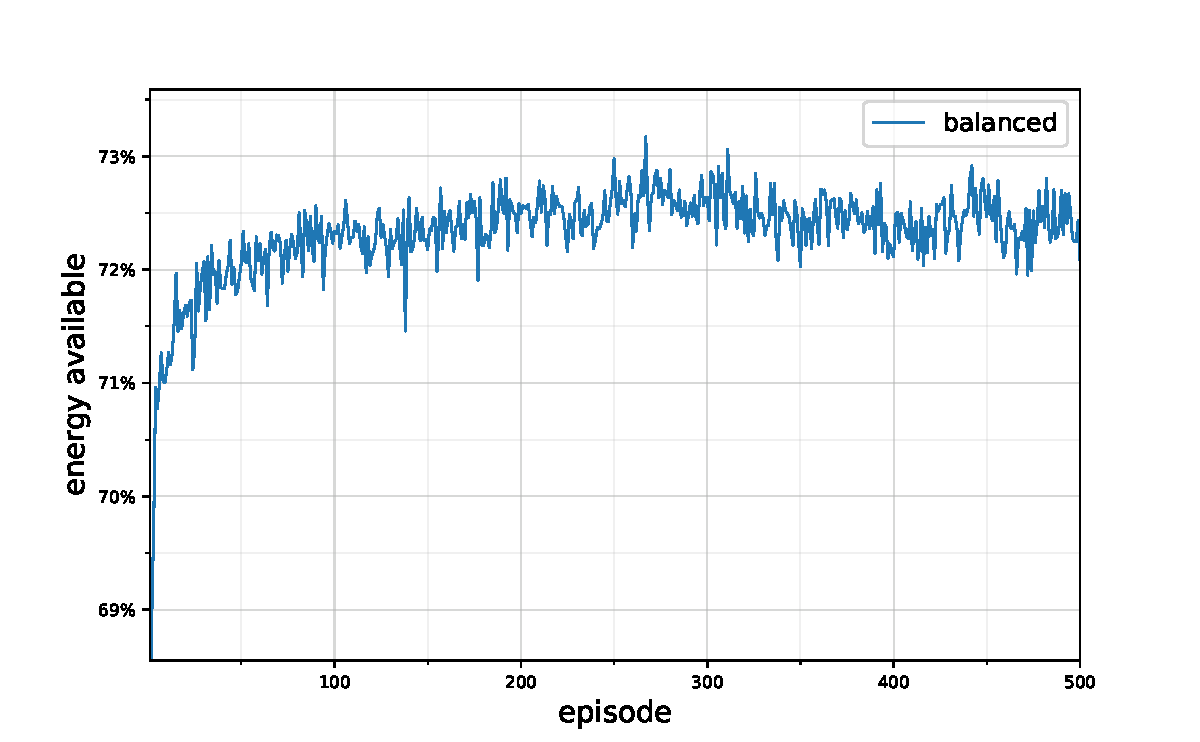
\includegraphics[width=0.7\linewidth]{5_ctv-statistics-energy-available}
	\captionsetup{labelfont=bf,singlelinecheck=on}
	\caption{Energy available in the system as percentage of the theoretical optimal}
	\label{fig:5_ctv-statistics-energy-available}
\end{figure}
\begin{figure}[ht]
	\centering
	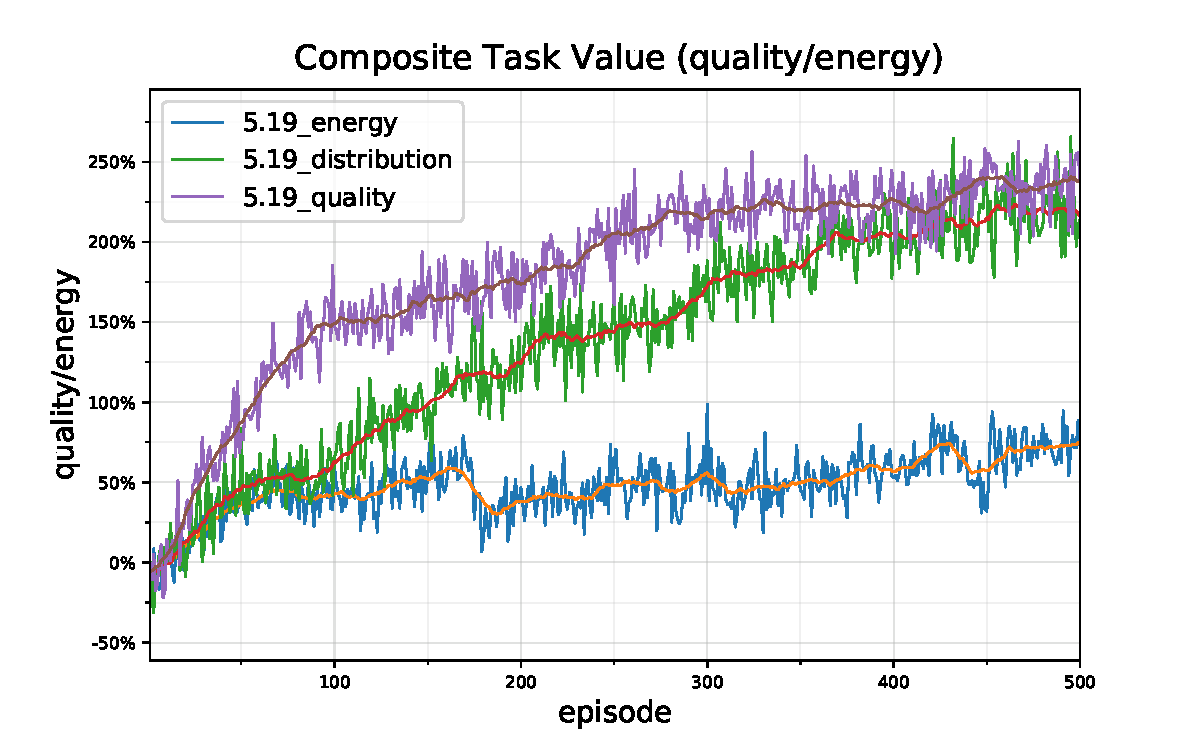
\includegraphics[width=0.8\linewidth]{5.19_ctv-quality-energy}
	\captionsetup{labelfont=bf,singlelinecheck=on}
	\caption{Quality compared to system optimal}
	\label{fig:5.19_ctv-quality-energy}
\end{figure}

\begin{figure}[ht]
	\centering
	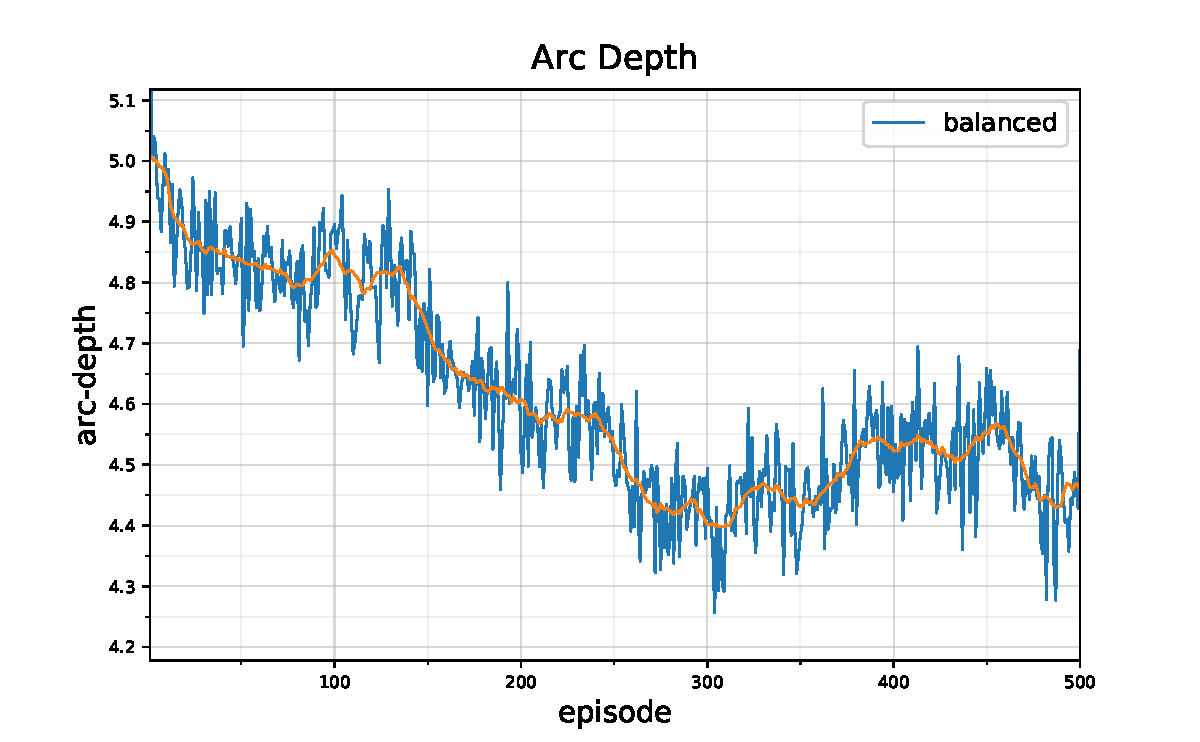
\includegraphics[width=0.7\linewidth]{5_ctv-arc-depth}
	\captionsetup{labelfont=bf,singlelinecheck=on}
	\caption{Arc depth}
	\label{fig:5_ctv-arc-depth}
\end{figure}
\begin{figure}[ht]
	\centering
	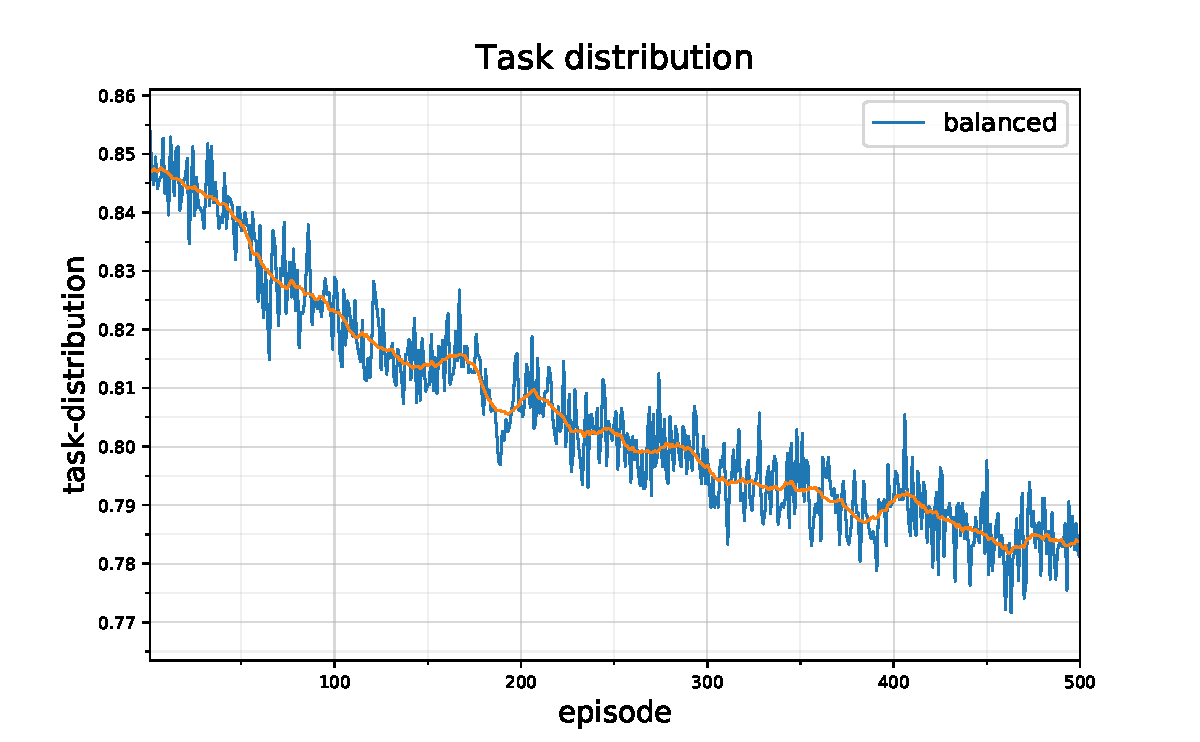
\includegraphics[width=0.7\linewidth]{5_ctv-task-distribution}
	\captionsetup{labelfont=bf,singlelinecheck=on}
	\caption{Task distribution}
	\label{fig:5_ctv-task-distribution}
\end{figure}
